\chapter{CERN, the LHC and LHCb}
%\cite{LHC}


%CERN section
%In this section I would like to introduce what CERN very briefly I an not sure if I want to mention much of it's history but I would like to mention LEP since the LHC was build in the LEP tunnel

%LHC section 
%Here I want to describe the LHC and briefly how it works along with the experiments which are on the LHC ring. I would also like to mention the different Runs that have occurred at the LHC and say how I will mention Run 2 and Run 3 since we shall elude to them and also some developments looked into were designed to be used in Run 2 or with Run 2 in mind. 

%LHCb section
%I shall descirbe what LHCb is, prehaps with a section for tracking and then the PID and I shall have a small section on the trigger (maybe here mention that there were changes in Run 2 but we don't use these for any analysis here and also that we don't want the turbo stream since we are a very rare decay. I think it may be nice to have a table of what luninoscities were collected since I can then later justify not using Run 2 data. Should maybe mention that we did do lead lead collisions for the first time though I didn't look at them (only did a shift).



%\section{CERN}

% Plan
%OUTLINE for CERN
%> began in 1954 with 12 memberstates, as a collaborative way for Europe for study nuclear physics, based in Genava Switzerland
%> The collabrative nature of CERN has allowed for largescale expensiveexperiments to be built
%> The PS was CERN's flagship accelerator which began operationsin 1959 and acceleratedprotonsto XXXeV and was 628m in circumference ( I could mention the SPS and LEP here too if that would make things fit better later on)
%> now 62 years later there are 21 member states as well as some others
%> and we have the LHC which is 27km in diameter and was designed to collide protons at 14 TeV and lead ions at 2.76 TeV per nucleon
%> Do I want to mention successes that have occured at CERN, do I want to show that I know that there are other experiments at CERN? Do I want to mention LEP since the LHC was built in the LEP tunnel? I think that I like what I have written so far and it is a very ver short CERN section therefore I think that as it is I should just have it as an introduction to the chapter. 



The European Organisation for Nuclear Research (CERN) was founded in 1954 and began with 12 member states as a organisation to encourage European collaboration and the study of nuclear physics. Since it's foundation the collaborative nature of CERN allowed for large-scale expensive experiments and machines to be built. The Proton Synchrotron was CERN's flagship accelerator, operational in 1959 it had a circumference of 628m and accelerated protons to XXX GeV the highest energy at that time. Now 62 years since it's foundation CERN has grown to include 21 member states \footnote{about the other types of countries involved.} and it’s latest accelerator, the Large Hadron Collider (LHC), is most energetic particle accelerator ever built, with a 27km circumference the LHC was designed to protons at 14 TeV.
This chapter shall discuss the LHC and the LHC beauty experiment, one of the experiments that uses collisions provided by the LHC.



\section{The LHC}

Introduction of what the LHC is and what it was designed to do
> The Large Hadron Collider was conveived in 1980 with the purpose to test the SM, look for the Higgs and the capabilities to allow for probbing beyond the SM
> it was built in the LEP tunnel for cost reasons - therefore 27km long
> It is a synchrotron
> It accelerates and collides protons and also lead ions
> Two main things to consider for a accelerator are the lumi and energy, explain what lumi is
> The LHC was degined to run at an energy of 14 TeV and 10^34cm-2s-1 lumi and 25ns bunches w XXX protons per bunch

> the are 4 interaction points where where the LHC makes it's beams collides and the results of these collisions are studied


How does the LHC work, acheive it's objectives
> The LHC gets its protons from a chain of other accelerators
> The PS and SPS have been modified several times over the years to provide for larger accelerators
> The linac 2 was designed just to get stuff for other experiments
> The LHC accelerates it's protons with RF cavities, bends with dipole magnets and focus with quadrapole magnets
> There are 2 beams that rotate in oposite directions
> in order to get the 14TeV 8T magnets had to be used - this limits the lead energy to 2.76 TeV
> collisions occur

OR

> LHC is a synchrotron to look at SM, Higgs and BSM
> is was built in the LEP tunnel
> The LHC was designed to collide hadrons - protons at 14TeV with 4 interaction points with lumi of 10^34cm-2s-1
> lumi is XXXX and is acheived by the number of protons in the bunches and time between the bunches
> This is how is works RF accelerate, dipoles bend (have to be 8.3T for 27km and 14 TeV) quadrapoles focus for the interaction points
> But where does it get the protons from, Linac2, PSB, PS, SPS
> although there is space in the LHC for X bunches - there can only be Y due to the accelerator chain
> It can also collide lead ions but I'm not interested in this (so it's not covered in detail) but the 8T magnets limit the lead ions to 2.76 TeV/nucleon

What has happened at the LHC so far
> It ran from 2010 - 2013 had LS2 then started up again in 2015 at a higher energy
> What I am interested in for this thesis


What looks at the collisions
> ATLAS  - A Totally Ludicrous AparatuS
> CMS - Crap Muon Solenoid, sorry what solenoid
> TOTEM - TOTally umEMportant
> LHCf - LHC forgotten
> MoEDAL - 
> ALICE - 
> LHCb - where the b is clearly for best!



Then power on to LHCb

Start
> Introduces LHCb briefly
> explain what the coordinated I shall use are
> mention LS2 and Run 2 and stuff

Tracking

PID

Trigger

Stripping

Runs for LHCb


%\section{CERN}





\section{The LHC Machine}

The Large Hadron Collider (LHC) \cite{LHC} is a two beams collider predominately designed to collide protons at an energy of 14 T$e$V but the accelerator can also study collisions of heavy ions. 
It has been built on the Franco-Swiss border in the tunnel previously used for the LEP machine at CERN\footnote{CERN is the 
European Organisation for Nuclear Research.} with the aim of studying predictions of the Standard Model of particle physics and looking for New Physics beyond the
Standard Model. The LHC is the last element of an
accelerator complex shown in Fig.~\ref{LHC}: accelerators previously used at CERN have been modified in order to supply the LHC with high density proton bunches. Protons are first accelerated in the Linac 2 to an energy of 50MeV, 
the then pass through the Proton Synchrotron Booster, Proton Synchrotron and the Super Proton Synchrotron reaching and energy of 450 GeV before injection into the LHC where they are accelerated
up to final energy. 

The LHC began taking data in December 2009, most of the data has been acquired during the runs in 2011 and 2012 at center of mass energies of 7 T$e$V and 8 T$e$V, respectively, with 50 ns between proton bunches. It is currently in downtime undergoing upgrades and shall resume
operation 2015 colliding proton bunches with a spacing of $25$ ns at a center of mass energy of 13 T$e$V. 


\section{The Experiments}
There are four detectors at the LHC, ATLAS, CMS, ALICE and LHCb, placed where the two beams cross over. The ATLAS \cite{ATLAS} and CMS \cite{CMS} detectors are general purpose detectors with 4$\pi$ angular acceptance 
and have been designed to perform general searches for New Physics and the Higgs boson.\footnote{ATLAS and CMS both discovered a possible candidate for the Standard Model Higgs in 2013 \cite{Higgs_ATLAS, Higgs_CMS}.}
The ALICE \cite{ALICE} detector is specialised to study heavy ion collisions in order to investigate strongly interacting matter and quark-gluon plasmas. The LHCb \cite{LHCb} detector is a single-arm spectrometer designed 
for the study of B-hadron decays.





\begin{figure}[h!]
\centering
  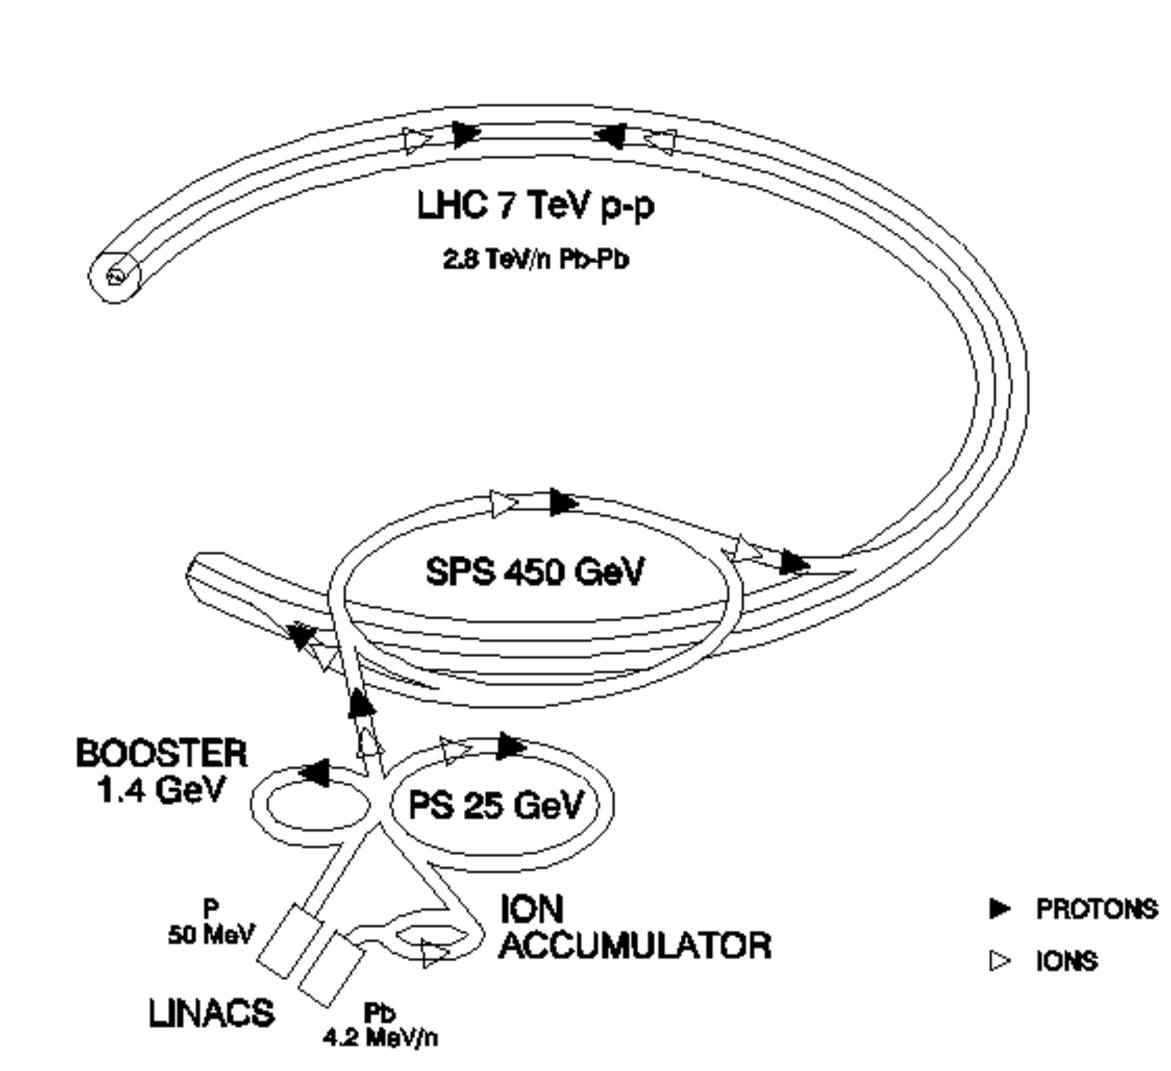
\includegraphics[width = 0.6 \linewidth]{accelerator_complex.pdf}
  \caption{The LHC and adjoining accelerator chain at CERN \cite{LHC}}
  \label{LHC}
\end{figure}

%The first run in 2009 caused the connections bwtn 2 magnets to lose their superconductivityness and this broke the detector, the magnets couldn't bend enough.
%They then checked all the other connections and it turned out that they weren't all great, but could couple with the current required to get bending for 7 and the 8 TeV.
%They have/are/will all now been re-done for 14 TeV.

%Also at 14TeV the time btwn bunches will be 25ns rather than the previous 50ns. It was built for 25 ns.

%The collider complex is needed to give proton bunches with high density and get them up at a suitable minimum energy.
%The bunches have slightly different accelerations given to them in the LHC to keep them as bunches. There for it's an oscillating electric field that accelerates them.
%This field has a max and min depending on the initial and final energies. The min can't be too low so bunches must start with some energy.
